\documentclass[a4paper, 11pt,table]{article}

\usepackage[utf8]{inputenc}
\usepackage[T1]{fontenc}
\usepackage[toc,page]{appendix}
\usepackage{varioref}
\usepackage{hyperref}
\usepackage[nameinlink]{cleveref}
\usepackage{nameref}
\usepackage{parskip}
\usepackage{multicol}%multi column bib
\usepackage[sectionbib, tocbib, numberedbib, bibnewpage]{apacite}%Citations
\usepackage{tikz}
\usepackage{pdflscape}
\usepackage{tabu}
\usepackage{pgfplots}
\usepackage[margin=0.5in]{geometry}

\usepackage{comment}
\excludecomment{figure}
\let\endfigure\relax

\pagenumbering{gobble}

\author{Steven Lowes}
\title{Software Methodologies AI Search}
\date{\today{}}

\newcommand{\smartref}[1]{%
	\hyperref[#1]{\cref{#1}, ``\nameref{#1}", \vpageref{#1}}%
}

\begin{document}
	
	\section{Algorithm A: Simulated Annealing}
	
	\subsection{Results}
	\begin{figure}
	\label{useCase:annealResults}
	\begin{center}
		\rowcolors{0}{gray!25}{white}
		\begin{tabu}{|c c c|}
			\textbf{Nodes} & \textbf{Tour Length} & \textbf{Runtime} \\
			12 & 56.0 & 0.11s \\
			17 & 1,514 & 2.42s \\
			21 & 2,716 & 2.46s \\
			26 & 1,487 & 9.08s \\
			42 & 1,217 & 9.64s \\
			48 & 14,846 & 14.66s \\
			58 & 26,740 & 13.95s \\
			175 & 21,613 & 2m10s \\
			180 & 2,720 & 2m16s \\
			535 & 50,191 & 13m23s \\
		\end{tabu}
	\end{center}
\end{figure}
	
	\subsection{Description}
	Simulated annealing is similar to a hill climbing algorithm, except it will occasionally move down the hill. The chance of doing so decreases as the algorithm nears completion.
	
	Each potential next state is selected with chance $e^{-(newValue - currentValue) / temperature}$
	
	\subsection{Start Temp}
	When the Start Temperature is too high, the simulation will frequently jump to worse states in the beginning. This means that the algorithm does not even begin to converge until it is a significant way through. To set the start temperature, i ran the algorithm with a very high start temperature, roughly 100,000. I set the algorithm to print out its progress while running, and noted that it appeared to begin to converge around 50 temperature. Knowing this, I experimented with different start temperatures, looking at the results. I found that approximately 70 start temperature was the lowest I could go without adversely affecting the results.
	
	
	\begin{figure}
	\begin{center}%TODO
		Using an end temp of 0.01:
		\rowcolors{0}{gray!25}{white}
		\begin{tabu}{|c c c|}
			\textbf{Start Temp} & \textbf{Tour Length} & \textbf{Runtime} \\
			10,000 & 55,111 & 1.99s \\
			5,000 & 53,643 & 8.40s \\
			1,000 & 52,678 & 23.2s \\
			500 & 50,928 & 1m15s \\
			100 & 50,301 & 3m25s \\
			75 & 50,191 & 13m23s \\
			50&&\\
			25&&\\
			10&&\\
			1&&\\
		\end{tabu}
	\end{center}
\end{figure}
	
	\subsection{End Temp}
	When the End Temperature is very low, the algorithm will spend a long time in a local minima, looking for a better result without ever jumping to a worse result. I set a very low end temperature, around 0.00001, and watched its progress. It was clear that below approximately 1 temperature, the algorithm was no longer improving its guess. Again, I experimented with a few different End Temperatures and found that a value of 1 was the best.
	
\begin{figure}
	\begin{center}%TODO
		Using a start temp of 10000:
		\rowcolors{0}{gray!25}{white}
		\begin{tabu}{|c c c|}
			\textbf{End Temp} & \textbf{Tour Length} & \textbf{Runtime} \\
			1,000 & 55,111 & 1.99s \\
			500 & 53,643 & 8.40s \\
			100 & 52,678 & 23.2s \\
			50 & 50,928 & 1m15s \\
			25 & 50,301 & 3m25s \\
			10 & 50,191 & 13m23s \\
			5&&\\
			2.5&&\\
			1&&\\
			0.5&&\\
			0.1&&\\
			0.01&&\\
			0.001&&\\
		\end{tabu}
	\end{center}
\end{figure}
	
	\subsection{Multithreading}
	Multithreading was implemented into my Simulated Annealing Algorithm. However, I never found a way to make it viable as a way to improve speed while keeping the results of equal quality. The way that I implemented multithreading was to run the simulation in `stages'. Each stage ran the same as the normal simulation, but with the number of steps split between the threads. The stage was run simulatenously on multiple threads. After $x$ steps were complete, the best result found from any of the stages was taken as the new best result, and the temperature updated.
	
	This meant that if $x$ was set too high, then the simulation would be very coarse. If it was set too low, then there would be a very large overhead from creating and destroying new threads. I was not able to find a value in the middle which sped up computation while keeping results of the same quality, or even close. It was quicker just to run the simulation on a single thread but with a quicker cooling rate, and you get results that are equally bad.
	
	On simulations which take weeks, it would probably make sense to enable this method of multithreading. You could set a very high $x$ value, and still get good results. This is becuase the overhead of generating the threads reduces as $x$ increases, but the negative effects on the results is proportional to $steps/x$.
	
	You can show that this method is flawed through \emph{reductio ad absurdum}. Increase the number of steps between each sync to be equal to the $n/cpus$ where $n$ is the total number of steps. Essentially, this method must reduce the quality of results because the alternative is that running annealing 10 times and taking the best result is just as good as running it once with 10 times as many steps.
	
	\subsection{Cooling Rate}
	The cooling rate can be changed via a parameter. The cooling rate is equal to $1-f$ where $f$ is the factor by which the temperature is multiplied by after each iteration. High cooling rates means that the simulation runs quicker but more coarsely, producing worse results. Conversely, low cooling rate means that the simulation takes more time, but produces better results. Runtime scales linearly with the number of steps.
	
\begin{figure}
	\begin{center}
		\rowcolors{0}{gray!25}{white}
		\begin{tabu}{|c c c|}
			\textbf{Steps (m)} & \textbf{Tour Length} & \textbf{Runtime} \\
			6.6 & 55,111 & 1.99s \\
			33 & 53,643 & 8.40s \\
			99 & 52,678 & 23.2s \\
			331 & 50,928 & 1m15s \\
			893 & 50,301 & 3m25s \\
			2,648 & 50,191 & 13m23s \\
		\end{tabu}
	\end{center}
\end{figure}

\begin{figure}
	\begin{center}
		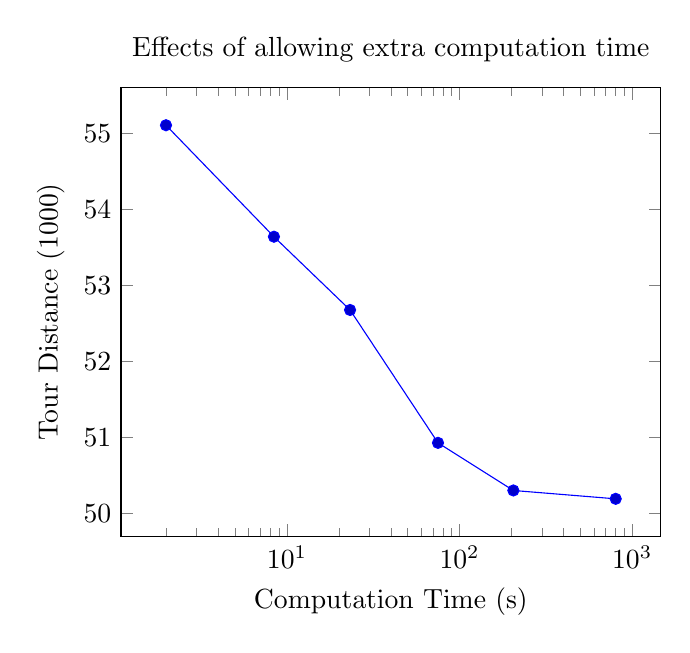
\begin{tikzpicture}
		\begin{axis}[
		title = Effects of allowing extra computation time,
		xlabel = {Computation Time (s)},
		ylabel = {Tour Distance (1000)},
		xmode=log,
		]
		\addplot coordinates {
			(1.99,55.111)
			(8.40,53.643)
			(23.2,52.678)
			(75,50.928)
			(205,50.301)
			(803,50.191)
		};
		\end{axis}
		\end{tikzpicture}
	\end{center}
\end{figure}

\begin{figure}
	\begin{center}
		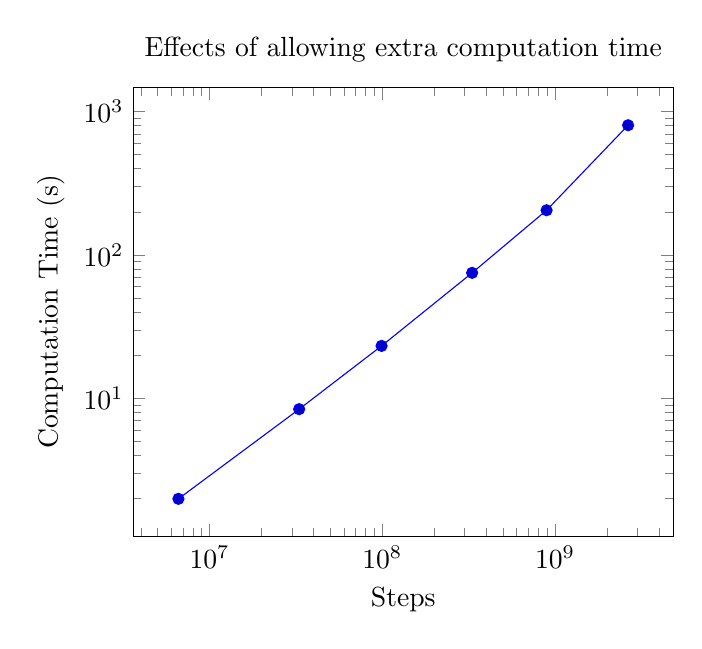
\begin{tikzpicture}
		\begin{axis}[
		title = Effects of allowing extra computation time,
		xlabel = {Steps},
		ylabel = {Computation Time (s)},
		xmode=log,
		ymode=log,
		]
		\addplot coordinates {
			(6600000,1.99)
			(33000000,8.40)
			(99000000,23.2)
			(331000000,75)
			(893000000,205)
			(2648000000,803)
		};
		\end{axis}
		\end{tikzpicture}
	\end{center}
\end{figure}
	
	\section{Algorithm B: Ant Colony Optimisation}
	
	\subsection{Results}
\begin{figure}
	\label{useCase:antResults}
	\begin{center}
		\rowcolors{0}{gray!25}{white}
		\begin{tabu}{|c c c|}
			\textbf{Nodes} & \textbf{Tour Length} & \textbf{Runtime (s)} \\
			12 & 56.0 & 0.60s \\
			17 & 1,444 & 1.02s \\
			21 & 2,549 & 1.28s \\
			26 & 1,575 & 2.98s \\
			42 & 1,322 & 6.27s \\
			48 & 12,702 & 15.72s \\
			58 & 25,855 & 19.10s \\
			175 & 21,770 & 2m25s \\
			180 & 1,950 & 3.42s \\
			535 & 53,409 & 9.4ss \\
			535 & 50,762 & 1m4s \\
			535 & 50,124 & 11m16s \\
		\end{tabu}
	\end{center}
\end{figure}
	
	\begin{figure}
	\begin{center}
		No Improvement after 100 iterations = convergence
		
		Iterations = 112 means that the best path was discovered on iteration 12
		
		\rowcolors{0}{gray!25}{white}
		\begin{tabu}{|c c c c|}
			\textbf{Ants} & \textbf{Iterations to Converge} & \textbf{Runtime} & \textbf{Tour Length} \\
			1 & 822 & 14.3s & 77,724 \\
			2 & 1015 & 21.2s & 69,213 \\
			4 & 905 & 26.2s & 63,728 \\
			8 & 410 & 18.3s & 62,443 \\
			16 & 429 & 34.9s & 59,890 \\
			32 & 372 & 60.8s & 58,620 \\
			64 & 315 & 1m17s & 58,031 \\
			128 & 364 & 2m55s & 57,445 \\
			256 & 167 & 2m56s & 56,773 \\
			512 & 110 & 34.11s & 55,426 \\
			1,024 & 112 & 1m10s & 53,729 \\
			2,048 & 106 & 2m20s & 52,571 \\
			4,096 & 106 & 4m36s & 51,674 \\
			8,192 & 104 & 8m40s & 51,197 \\
			16,384 & 104 & 15m52s & 50,709 \\
		\end{tabu}
	\end{center}
\end{figure}
	
	\subsection{Description}
	Ant Colony Optimisation simulates a number of ants moving around the graph. At each junction the ant chooses an edge to travel down using a weighted random selection. The weights for each edge are $Pheremones^{2}*Length^{-2}$. Shorter edges are more desirable, as are edges with more pheremones. After each iteration, all ants deposit pheremones on the paths they travelled down. Pheremones then evaporate, with the pheremones on each edge being multiplied by a constant factor.
	
	\subsection{Elite Ant}
	In each iteration, the best all-time ant was added to the ants to be processed. This means that the best all-time path has pheremones deposited onto it after each iteration, even if none of the generated ants chose that path.
	
\begin{figure}
	\begin{center}
		Elite Ant
		
		\rowcolors{0}{gray!25}{white}
		\begin{tabu}{|c c c c c|}
			\textbf{Ants} & \textbf{Iterations (With)} & \textbf{Iterations (W/O)} & \textbf{Length(With)} & \textbf{Length (W/O)} \\
			 2 & 839 & 1184 & 68,531 & 69,758 \\
			 4 & 565 & 784 & 64,445 & 64,362 \\
			 8 & 474 & 505 & 61,375 & 61,137 \\
			 16 & 444 & 505 & 59,612 & 59,553 \\
			 32 & 310 & 397 & 58,710 & 58,582 \\
			 64 & 111 & 221 & 58,401 & 57,755 \\
			 128 & 250 & 219 & 56,159 & 57,615
		\end{tabu}
	\end{center}
\end{figure}
	
	The algorithm with the Elite Ant consistently outperforms the algorithm without the Elite Ant, albeit marginally. The Elite Ant algorithm ranges from slightly faster to much faster, and the tour lengths are well within the margin of error.
	
	\subsection{Multithreading}
	Implementing multithreading into the ant colony optimisation was very easy and does not reduce the quality of the results whatsoever. When generating the ant population, simply create multiple threads and ask each thread to create a portion of the ants. We then combine the generated lists and process the ants in a single-threaded manner. This works due to the fact that the during the generation of the ants, the shared resources are processed in an entirely read-only fashion. It is not necessary to run the ant processing in parallel because it is a small fraction of the total computation performed. The processing step could be run in parallel in future but this will be more difficult to implement due to shared resources being mutated.
	
\begin{figure}
	\begin{center}
		Normalised so that ST and MT assume same amount of iterations
		
		\rowcolors{0}{gray!25}{white}
		\begin{tabu}{|c c c|}
			\textbf{Ants} & \textbf{Runtime (Single Thread)} & \textbf{Runtime (Multithread)} \\
			16 & 34.9s & 11.4s \\
			32 & 60.8s & 12.2s \\
			64 & 1m17s & 16.6s \\
			128 & 2m55s & 39.7s \\
			256 & 2m57s & 26.1s \\
			512 & 3m36s & 38.3s \\
			1,024 & 6m49s & 1m8s \\
			2,048 & 13m22s & 2m8s \\
		\end{tabu}
	\end{center}
\end{figure}
	
	\subsection{Culling}
	I attempted to improve performance of the ant colony optimisation by culling edges with sufficiently low desirability. This would mean that culled edges did not need to be considered when performing the weighted random selection. However, there was not a happy medium between having the culling happen to early (and therefore reduce the quality of the results) and having it happen too late (by which point the algorithm had already converged and we could have just ended it immediately).
	
\begin{figure}
	\begin{center}
		\rowcolors{0}{gray!25}{white}
		\begin{tabu}{|c c c|}
			\textbf{Culling Rate (\% of remaining edges per iteration)} & \textbf{Iterations} & \textbf{Tour Length} \\
			0 & 163 & 57,154 \\
			0.1 & 144 & 57,700 \\
			0.5 & 69 & 59,838 \\
			1 & 35 & 62,910 \\
			5 & 9 & 76,6992 \\
			10 & 4 & 84,099 \\
		\end{tabu}
	\end{center}
\end{figure}
	
	\subsection{Termination Criteria}
	We terminate after no improvement for $x$ iterations. This is set at 10. It's rare that after 10 iterations with no improvement that you will suddenly see improvement - what tends to happen is just that all the ants converge onto the current best path and stay there.
	
	With more ants we tend to converge within less than 10 steps. With fewer ants we need to increase the number because it can 50+ iterations to see any improvement.
	
	\section{General}
	\subsection{Fast Triangular Array}
	The original way that I stored the matrix was using a HashMap of unordered pairs. This was horrifically slow. Accessing the length of an edge meant creating a new object, hashing it, then retrieving that from the hashtable. I moved to a much faster method, using a contiguous block of memory. I created an array of $size=nodes^2$. When requesting position $(x,y)$, it retrieved position $x_2 \times nodes + y_2$ where $x_2$ was $min(x,y)$ and $y_2$ was $max(x,y)$. This reflects the directionless nature of the graph.
	
	\subsection{Grouping}
	If we group nodes that are close to each other into groups, we can treat each group as a node in a new network. From here, we can solve the new network, and then solve each group. This can be done recursively --- we can have groups of groups of groups etc.
	
	This doesn't work well on the size of networks that we are dealing with. It would potentially have merit with very large networks, with millions or billions of nodes, where there is no chance of ever getting close to optimal. It also relies on the fact that the network is created in euclidean space, meaning that if nodes A and B are close to node C, and C is close to D, then the direct path from A and B to D is no longer than the path going through C.
	
	Choosing how to group the nodes is the main challenge with this technique. The optimal grouping would minimise the sum of the optimal TSP tours for each group. However, this obviously isn't feasible as this brute force approach would take $n! \times n \times (n/m)!$ as opposed to just solving the original TSP which only takes $n! \times n$ (where $n$ is the number of nodes and $m$ is the number of groups)
	
	When generating the new network from the graph, we need to generate edges and distances for those edges. It is difficult to know what value to use for the distances, as they need to accurately represent how difficult it is to move from one group to another.

\begin{figure}
	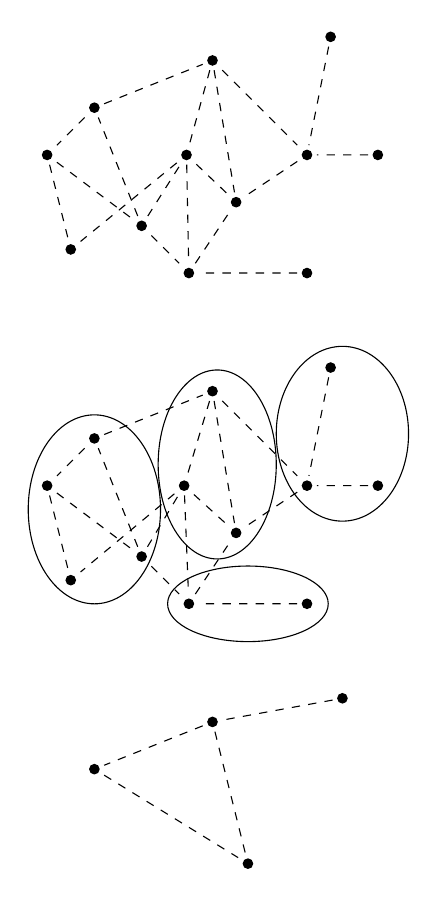
\begin{tikzpicture}[rotate=180,scale=0.6]
	\node (v4) at (-4,-20.5) {};
	\node (v5) at (-4.95,-22) {};
	\node (v7) at (-2,-22) {};
	\node (v8) at (-2.5,-20) {};
	\node (v6) at (-3,-23) {};
	\node (v2) at (-5,-19.5) {};
	\node (v11) at (-7.5,-22) {};
	\node (v9) at (-5.5,-24) {};
	\node (v3) at (-6,-21) {};
	\node (v1) at (-7.5,-19.5) {};
	\node (v10) at (-8,-24.5) {};
	\node (v12) at (-9,-22) {};
	
	\draw (v4) [fill=black] ellipse (0.1 and 0.1);
	\draw (v5) [fill=black] ellipse (0.1 and 0.1);
	\draw (v7) [fill=black] ellipse (0.1 and 0.1);
	\draw (v8) [fill=black] ellipse (0.1 and 0.1);
	\draw (v6) [fill=black] ellipse (0.1 and 0.1);
	\draw (v2) [fill=black] ellipse (0.1 and 0.1);
	\draw (v11) [fill=black] ellipse (0.1 and 0.1);
	\draw (v9) [fill=black] ellipse (0.1 and 0.1);
	\draw (v3) [fill=black] ellipse (0.1 and 0.1);
	\draw (v1) [fill=black] ellipse (0.1 and 0.1);
	\draw (v10) [fill=black] ellipse (0.1 and 0.1);
	\draw (v12) [fill=black] ellipse (0.1 and 0.1);
	
	\draw [dashed] (v1) edge (v2);
	\draw [dashed] (v2) edge (v3);
	\draw [dashed] (v4) edge (v5);
	\draw [dashed] (v4) edge (v6);
	\draw [dashed] (v7) edge (v8);
	\draw [dashed] (v7) edge (v4);
	\draw [dashed] (v5) edge (v2);
	\draw [dashed] (v4) edge (v2);
	\draw [dashed] (v9) edge (v5);
	\draw [dashed] (v10) edge (v11);
	\draw [dashed] (v12) edge (v11);
	\draw [dashed] (v11) edge (v3);
	\draw [dashed] (v9) edge (v11);
	\draw [dashed] (v6) edge (v7);
	\draw [dashed] (v5) edge (v8);
	\draw [dashed] (v5) edge (v3);
	\draw [dashed] (v9) edge (v3);
	\draw [dashed] (v6) edge (v9);
	
	\node (v4) at (-4,-13.5) {};
	\node (v5) at (-4.9,-15) {};
	\node (v7) at (-2,-15) {};
	\node (v8) at (-2.5,-13) {};
	\node (v6) at (-3,-16) {};
	\node (v2) at (-5,-12.5) {};
	\node (v11) at (-7.5,-15) {};
	\node (v9) at (-5.5,-17) {};
	\node (v3) at (-6,-14) {};
	\node (v1) at (-7.5,-12.5) {};
	\node (v10) at (-8,-17.5) {};
	\node (v12) at (-9,-15) {};
	
	\draw (v4) [fill=black] ellipse (0.1 and 0.1);
	\draw (v5) [fill=black] ellipse (0.1 and 0.1);
	\draw (v7) [fill=black] ellipse (0.1 and 0.1);
	\draw (v8) [fill=black] ellipse (0.1 and 0.1);
	\draw (v6) [fill=black] ellipse (0.1 and 0.1);
	\draw (v2) [fill=black] ellipse (0.1 and 0.1);
	\draw (v11) [fill=black] ellipse (0.1 and 0.1);
	\draw (v9) [fill=black] ellipse (0.1 and 0.1);
	\draw (v3) [fill=black] ellipse (0.1 and 0.1);
	\draw (v1) [fill=black] ellipse (0.1 and 0.1);
	\draw (v10) [fill=black] ellipse (0.1 and 0.1);
	\draw (v12) [fill=black] ellipse (0.1 and 0.1);
	
	\draw [dashed] (v1) edge (v2);
	\draw [dashed] (v2) edge (v3);
	\draw [dashed] (v4) edge (v5);
	\draw [dashed] (v4) edge (v6);
	\draw [dashed] (v7) edge (v8);
	\draw [dashed] (v7) edge (v4);
	\draw [dashed] (v5) edge (v2);
	\draw [dashed] (v4) edge (v2);
	\draw [dashed] (v9) edge (v5);
	\draw [dashed] (v10) edge (v11);
	\draw [dashed] (v12) edge (v11);
	\draw [dashed] (v11) edge (v3);
	\draw [dashed] (v9) edge (v11);
	\draw [dashed] (v6) edge (v7);
	\draw [dashed] (v5) edge (v8);
	\draw [dashed] (v5) edge (v3);
	\draw [dashed] (v9) edge (v3);
	\draw [dashed] (v6) edge (v9);
	\draw (-8.25,-16.1) node (v21) {} ellipse (1.4 and 1.85);
	\draw (-6.25,-12.5) node (v22) {} ellipse (1.7 and 0.8);
	\draw (-3,-14.5) node (v24) {} ellipse (1.4 and 2);
	\draw (-5.6,-15.45) node (v23) {} ellipse (1.25 and 2);
	
	\node (v13) at (-8.25,-10.5) {};
	\node (v14) at (-5.5,-10) {};
	\node (v16) at (-3,-9) {};
	\node (v15) at (-6.25,-7) {};
	
	\draw (v13) [fill=black] ellipse (0.1 and 0.1);
	\draw (v14) [fill=black] ellipse (0.1 and 0.1);
	\draw (v16) [fill=black] ellipse (0.1 and 0.1);
	\draw (v15) [fill=black] ellipse (0.1 and 0.1);
	
	\draw [dashed] (v13) edge (v14);
	\draw [dashed] (v14) edge (v15);
	\draw [dashed] (v16) edge (v15);
	\draw [dashed] (v14) edge (v16);
	\end{tikzpicture}
\end{figure}
\end{document}
